\documentclass[russian,english,hyperref=unicode]{beamer}

\usepackage{cmap}
\usepackage[utf8]{inputenc}
\usepackage[T1]{fontenc}
\usepackage{tabularx}
\usepackage{listings}
\usepackage[russian,english]{babel}
\usepackage{mathptmx}
\usepackage{multimedia}
\usepackage{amsmath}
\usepackage{amsthm}
\usepackage{graphicx}
\usepackage{amssymb}

%LST LISTINGS
\usepackage{listings}
\usepackage{tikz,pgfplots}
%\pgfplotsset{compat=newest}
%\pgfplotsset{plot coordinates/math parser=false}

\usepackage{color}
\definecolor{gray}{rgb}{0.4,0.4,0.4}
\definecolor{darkblue}{rgb}{0.0,0.0,0.6}
\definecolor{cyan}{rgb}{0.0,0.6,0.6}

\lstset{
  showstringspaces=false,
  commentstyle=\color{gray}\upshape,
  basicstyle=\footnotesize,
  columns=flexible,
  frame=single,
  breaklines=true,
  frame=multipled
}

\lstdefinelanguage{XML}
{
  morestring=[b]",
  morestring=[s]{>}{<},
  morecomment=[s]{<?}{?>},
  stringstyle=\color{black},
  identifierstyle=\color{darkblue},
  keywordstyle=\color{cyan},
  morekeywords={xmlns,version,type}% list your attributes here
}


\usepackage[absolute,overlay]{textpos}
\usepackage[labelformat=empty]{caption}

%\usetheme{Darmstadt}...
\usetheme{default}
\usecolortheme{dove}
\usenavigationsymbolstemplate{}
\setbeamertemplate{footline}{}

 % BigIMgH
\newcommand<>{\bigimgh}[2]{
        {
          \begin{frame}{#2}
                        \begin{tikzpicture}[remember picture]
                                \node[at=(current page.center)] {
                                        \includegraphics[height=\paperheight]{#1}
                                };
                        \end{tikzpicture}
                \end{frame}
        }
}
 % BigIMg
\newcommand<>{\bigimg}[2]{
        {
          \begin{frame}{#2}
                        \begin{tikzpicture}[remember picture,overlay]
                                \node[at=(current page.center)] {
                                        \includegraphics[width=\paperwidth]{#1}
                                };
                        \end{tikzpicture}
                \end{frame}
        }
}


\author{Alexander Ulitin}
\begin{document}
\selectlanguage{russian}

% \title{ Сравнение подходов обучения на базе словаря и MAP к проблеме повышения разрешения на примере изображений автомобильных номеров }
\title{Super resolution of license plate images: comparative analysis of dictionary-based and MAP-based approaches}
\author{
  \begin{tabular}[4cm]{rl}
 Author:                & Ulitin A.~A. \\
 & alexander.a.ulitin@gmail.com\\
%R  Science supervisor: & Ph.D.~Vakhitov A.~T. \\
%R  & alex@divisionlabs.com \\
 \end{tabular}
 }
\date{Mathematics and Mechanics Faculty \\
  St. Petersburg State University \\
2013 year}

\begin{frame}{}
		\maketitle
\end{frame}

% \section{Задача}
% \begin{frame}{Задача Super-resolution}
%   Задача Super resolution --- качественно повысить разрешения изображения.
%   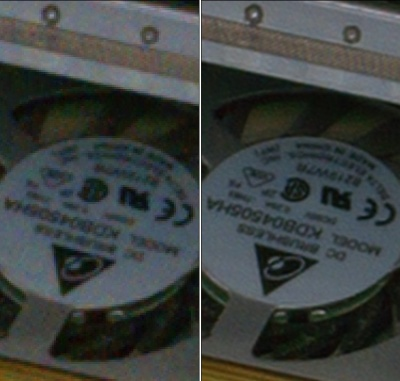
\includegraphics[height=\textheight]{content/An_example_of_super_resolution_with_still_RAW_photo.jpg}
% \end{frame}

\begin{frame}{Why is it possible}
  Image super-resolution use additional knowelege about enviroment:
  \begin{itemize}
    \item Knoweledge of blur information, camera motion etc
    \item Knoweledge of imaging object(text, faces, car plates, etc)
    \item Using several images taked from different places
  \end{itemize}

  Adaptability:
  \begin{itemize}
    \item Preprocessing for another CV algorythm.
    \item Extract additional information from several images.
  \end{itemize}
\end{frame}

\begin{frame}{Superresolution methods}
  \begin{itemize}
    \item Training algorithms
    \item Interpolation
    \item Spectral representation
    \item Regularization
  \end{itemize}

Or any combination of methods from above
\end{frame}

\begin{frame}{PSNR metric}

  $$ \mathrm{MSE}(\tilde{x},x) = \frac{1}{m\,n}\sum_{i=0}^{m-1}\sum_{j=0}^{n-1} [\tilde{x}(i,j) - x(i,j)]^2$$

  $\mathrm{PSNR}(\tilde{x},x)$.
  $$ \mathrm{PSNR}(\tilde{x},x) &= 10 \cdot \log_{10} \left( \frac{\mathrm{MAX}_I^2}{\mathrm{MSE}(\tilde{x},x)} \right)
  $$
  where $MAX_i$ -- maximum possible pixel value of the image.

\end{frame}

\begin{frame}{Problem formulation}
 $$y_r = D H_R W_R x + n_r,~ ~ ~ 1 \leq r \leq m$$
where:
 \begin{itemize}
\item $ x $ original image
\item $ y_r $ observation r    
\item $ D $ matrix downsampling    
\item $ W $ matrix of geometric distortion    
\item $ H_R $ matrix blur observation r    
\item $ n_r $ observation noise r    
\item $ m $ the number of observations
 \end{itemize}
 The task of finding:
 $$ \tilde{x} = \underset{\hat{x}}{\operatorname{argmax}}~  PSNR(\hat{x},x)$$
\end{frame}

\begin{frame}{Subpixel motion}
For subpixel motion we use bicubic interpolation between image pixels.

In our experiments we use model with shift, gaussian blur and normal distributed noise.
\end{frame}

\section{Methods}
\begin{frame}{Methods}
  \begin{itemize}
    \item Couple Dictionary Training for Image Super-resolution \\
        (Jianchao Yang,Zhaowen Wang, Zhe Lin,Scott Cohen, and Thomas Huang) \\
  The main idea is very simple - learn dictionary of small patches in two resolutions LR and HR.
      \begin{itemize}
        \item use two coupled dictionary
        \item super-resolution by 1 image
      \end{itemize}
    \item Superresolution of License Plates in Real Traffic Videos \\
      (K. V. Suresh, G. Mahesh Kumar, and A. N. Rajagopalan) \\
      Image to be superresolved is modeled as a Markov random field and is estimated from the observations by a graduated
nonconvexity optimization procedure.
      \begin{itemize}
        \item A discontinuity adaptive regularizer is used to preserve the
edges in the reconstructed number plate for improved readability.
      \end{itemize}
  \end{itemize}
\end{frame}

\begin{frame}{Couple Dictionary Training for Image Super-resolution}
  \begin{itemize}
    \item learn couple dictionaries relate the low- and high-resolution image patch

    \item we using author's implementation of algorithm with our training and test data.

  \end{itemize}
\end{frame}

\begin{frame}[allowframebreaks]{Superresolution of License Plates in Real Traffic Videos}
\begin{enumerate}
  \item Calculate $X^0$ as the average of the bilinearly upsampled and aligned images
  \item Choose a convex $\lambda = 2v$, where v is the maximum value of the gradient along the x and y directions in the
    initial estimate $X^0$
  \item Do:
    \begin{enumerate}
      \item $X^{(n+1)} = X^{(n)} - \alpha\cdot\mathrm{grad}(X^{(N)}, \gamma) $
      \item $n=n+1$
      \item If $(\operatorname{norm}(X^{(n)}-X^{(n-1)}) < \epsilon)$\\
        then $\gamma^{(n)} = \max \{\gamma_{\mathrm{target}}, k\gamma^{(n-1)}\}$
    \end{enumerate}
    Until $(norm(X^{(n)}-X^{(n-1)} < \epsilon)$ and $(\gamma^{(n)} = \gamma_{\mathrm{target}})$

  \item $ \hat{x} = X^{(n)}$
    where $\alpha$, $\epsilon$, $k$, $\gamma_{\mathrm target}$ experimentally selected parameters of the algorithm.
\end{enumerate}
$$
\mathrm{grad}(x, \gamma) = \frac{1}{\sigma^2} \sum^m_{r=1} W^T_R H^T_r D^T (D H_r W_r x-y_r) + \lambda \cdot G(x, \gamma)
$$
где $\lambda$experimentally chosen regularization parameter and the gradient to the point $ (i, j) $ is given by the
following formula:

$$
\begin{array}{rcl}
 G(i,j) & = & 2\left[x(i,j)-x(i,j-1)\right] \exp\left(-[ x(i,j)-x(i,j-1) ]^2/\gamma \right) \\
& + & 2\left[x(i,j)-x(i,j+1)\right] \exp\left(-[ x(i,j)-x(i,j+1) ]^2/\gamma \right) \\
& + & 2\left[x(i,j)-x(i+1,j)\right] \exp\left(-[ x(i,j)-x(i-1,j) ]^2/\gamma \right) \\
& + & 2\left[x(i,j)-x(i-1,j)\right] \exp\left(-[ x(i,j)-x(i+1,j) ]^2/\gamma \right)
\end{array}
$$
\end{frame}

%\section{Описание подходов}
%\begin{frame}{Подход с тренированными словарями}
%\end{frame}

% \newcommand{\inimage}[2]{
%   \begin{minipage}{#1}
%     \vcenter{\includegraphics[width=\columnwidth]{#2}}
%   \end{minipage}
% }
%
%
% \section{Приведение изображений}
% \begin{frame}{Несколько изображение $\rightarrow$ одно изображение}
%   Для тестирования на однинаковых наборах данных из lr строились псевдо hr для
%   первого алгоритма методом:
%   $$ R = \frac{1}{n}\sum_{i=1}^nW^T \cdot S \cdot IMG_{lr i}$$
%   $S$ --- билинейная интерполяция \\
%   $W$ --- сдвиг
%
%   \inimage{3cm}{content/imgs/append_imgs_big.jpg}
%   $\to$
%   \inimage{6cm}{content/imgs/combined_big.jpg}
% \end{frame}

\begin{frame}{The original images}
  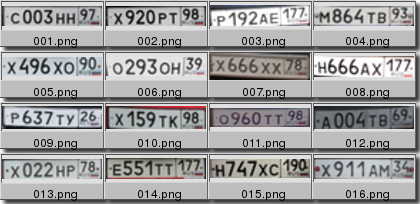
\includegraphics[width=\columnwidth]{content/out_sr1.png}
\end{frame}

\section{SR1}
\begin{frame}{The results of the algorithm with coupled dictionaries}
  % This file was created by matlab2tikz v0.3.3.
% Copyright (c) 2008--2013, Nico Schlömer <nico.schloemer@gmail.com>
% All rights reserved.
% 
% The latest updates can be retrieved from
%   http://www.mathworks.com/matlabcentral/fileexchange/22022-matlab2tikz
% where you can also make suggestions and rate matlab2tikz.
% 
% 
% 
\begin{tikzpicture}

\begin{axis}[%
width=10cm,
height=7.88709677419355cm,
scale only axis,
xmin=0,
xmax=16,
xlabel={Image number},
ymin=14,
ymax=28,
ylabel={PSNR dB},
legend style={draw=black,fill=white,legend cell align=left}
]
\addplot [
color=blue,
solid
]
table[row sep=crcr]{
1 22.6637207689603\\
2 16.5862621065916\\
3 20.2561814850212\\
4 16.8180326138836\\
5 15.2818944883097\\
6 20.8935173361133\\
7 19.9100975616132\\
8 21.8054095243458\\
9 19.5938529440994\\
10 14.97066690973\\
11 17.6444789637467\\
12 19.6591796988059\\
13 24.5276502442069\\
14 19.6886965973242\\
15 18.0639264824657\\
16 22.7687595823891\\
};
\addlegendentry{algorithm with coupled dictionaries};

\addplot [
color=green!50!black,
dashed
]
table[row sep=crcr]{
1 20.654183811932\\
2 15.5287572495406\\
3 14.6873141103361\\
4 16.906444307724\\
5 16.6431061328363\\
6 15.8814467785726\\
7 15.7004358294634\\
8 20.0170778439843\\
9 15.4643027107035\\
10 16.2470604606123\\
11 17.5627961112945\\
12 23.0775671820967\\
13 22.5057715768468\\
14 17.6125613605738\\
15 17.383467191801\\
16 16.1412027040119\\
};
\addlegendentry{Bicubic interpolation};

\end{axis}
\end{tikzpicture}%

\end{frame}

\begin{frame}{The results of the algorithm with coupled dictionaries}
  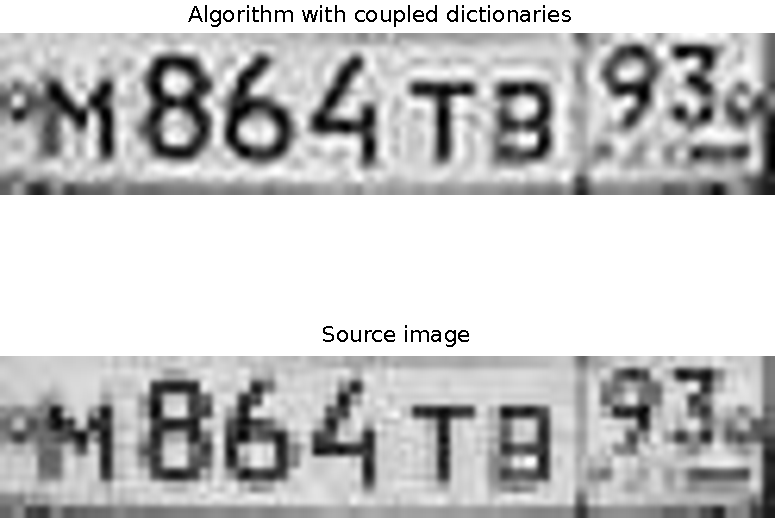
\includegraphics[width=\columnwidth]{content/compare_result_sr1_en.pdf}
\end{frame}

\section{SR2}
\begin{frame}{The results of algorithm FastSR}
  % This file was created by matlab2tikz v0.3.3.
% Copyright (c) 2008--2013, Nico Schlömer <nico.schloemer@gmail.com>
% All rights reserved.
% 
% The latest updates can be retrieved from
%   http://www.mathworks.com/matlabcentral/fileexchange/22022-matlab2tikz
% where you can also make suggestions and rate matlab2tikz.
% 
% 
% 
\begin{tikzpicture}

\begin{axis}[%
width=10cm,
height=7.88709677419355cm,
scale only axis,
xmin=0,
xmax=16,
xlabel={Image number},
ymin=12,
ymax=35,
ylabel={PSNR dB},
legend style={draw=black,fill=white,legend cell align=left}
]
\addplot [
color=blue,
solid
]
table[row sep=crcr]{
1 27.4470571608433\\
2 22.8300247931548\\
3 22.1109193658809\\
4 22.0652635937327\\
5 23.6272496813018\\
6 21.6055079117517\\
7 21.4619565703478\\
8 26.9867634881452\\
9 20.9809477047241\\
10 23.2957078121211\\
11 23.9394056382537\\
12 25.5317267141373\\
13 29.2416356490523\\
14 24.1599986234539\\
15 23.7307351145084\\
16 22.5888532577419\\
};
\addlegendentry{FastSR};

\addplot [
color=green!50!black,
dashed
]
table[row sep=crcr]{
1 18.4503335459593\\
2 15.9429403769346\\
3 15.9459841548511\\
4 15.5934814518383\\
5 16.9838249182421\\
6 13.7171337206461\\
7 12.7696291928783\\
8 21.6627180369299\\
9 13.6838913514568\\
10 18.8295593160528\\
11 17.4771261841067\\
12 20.0919833166445\\
13 22.2356695114555\\
14 16.697098012576\\
15 18.4542205359683\\
16 15.4386868770896\\
};
\addlegendentry{Bicubic interpolation};

\end{axis}
\end{tikzpicture}%

\end{frame}

\begin{frame}{The results of algorithm FastSR}
  % This file was created by matlab2tikz v0.3.3.
% Copyright (c) 2008--2013, Nico Schlömer <nico.schloemer@gmail.com>
% All rights reserved.
% 
% The latest updates can be retrieved from
%   http://www.mathworks.com/matlabcentral/fileexchange/22022-matlab2tikz
% where you can also make suggestions and rate matlab2tikz.
% 
% 
% 
\begin{tikzpicture}

\begin{axis}[%
width=5cm,
height=1cm,
axis on top,
scale only axis,
xmin=0.5,
xmax=50.5,
y dir=reverse,
ymin=0.5,
ymax=10.5,
hide axis,
name=plot1,
title={Initial estimation}
]
\addplot graphics [xmin=0.5,xmax=50.5,ymin=0.5,ymax=10.5] {../plots/sr2_psnr_rising-1.png};
\end{axis}

\begin{axis}[%
width=5cm,
height=1cm,
axis on top,
scale only axis,
xmin=0.5,
xmax=50.5,
y dir=reverse,
ymin=0.5,
ymax=10.5,
hide axis,
name=plot2,
at=(plot1.below south west),
anchor=above north west,
title={Original image}
]
\addplot graphics [xmin=0.5,xmax=50.5,ymin=0.5,ymax=10.5] {../plots/sr2_psnr_rising-2.png};
\end{axis}

\begin{axis}[%
width=5cm,
height=3.74020102770053cm,
scale only axis,
xmin=0,
xmax=60,
xlabel={Iteration},
ymin=12,
ymax=20,
ylabel={PNSR dB},
name=plot4,
at=(plot2.right of south east),
anchor=left of south west,
title={PSNR}
]
\addplot [
color=blue,
solid,
forget plot
]
table[row sep=crcr]{
1 12.3202813060895\\
2 12.9529644677536\\
3 13.5260641864726\\
4 14.0455567679328\\
5 14.5157791626175\\
6 14.9401084698002\\
7 15.3214501720298\\
8 15.6625515600167\\
9 15.966172416695\\
10 16.2351495750173\\
11 16.4723907826822\\
12 16.6808285374995\\
13 16.8633577505267\\
14 17.022773711704\\
15 17.1617200798005\\
16 17.2826512422842\\
17 17.3878096467359\\
18 17.4792164732515\\
19 17.5586729726292\\
20 17.6277695606153\\
21 17.6878999988837\\
22 17.7402784568312\\
23 17.7859577695793\\
24 17.8258476931939\\
25 17.8607323650764\\
26 17.8912864943554\\
27 17.9180900396926\\
28 17.9416412935904\\
29 17.9623683983446\\
30 17.9806393834473\\
31 17.9967708494893\\
32 18.011035438794\\
33 18.0236682351711\\
34 18.0348722293508\\
35 18.0448229763448\\
36 18.0536725585498\\
37 18.0615529553497\\
38 18.0685789072431\\
39 18.0748503506304\\
40 18.0804544886167\\
41 18.0854675536173\\
42 18.0899563091761\\
43 18.0939793311617\\
44 18.0975881022909\\
45 18.1008279486261\\
46 18.1037388421964\\
};
\end{axis}

\begin{axis}[%
width=5cm,
height=1cm,
axis on top,
scale only axis,
xmin=0.5,
xmax=50.5,
y dir=reverse,
ymin=0.5,
ymax=10.5,
hide axis,
at=(plot4.above north west),
anchor=below south west,
title={Result}
]
\addplot graphics [xmin=0.5,xmax=50.5,ymin=0.5,ymax=10.5] {../plots/sr2_psnr_rising-3.png};
\end{axis}
\end{tikzpicture}%

\end{frame}

\begin{frame}{The results of algorithm FastSR}
  % This file was created by matlab2tikz v0.3.3.
% Copyright (c) 2008--2013, Nico Schlömer <nico.schloemer@gmail.com>
% All rights reserved.
% 
% The latest updates can be retrieved from
%   http://www.mathworks.com/matlabcentral/fileexchange/22022-matlab2tikz
% where you can also make suggestions and rate matlab2tikz.
% 
% 
% 
\begin{tikzpicture}

\begin{axis}[%
width=5cm,
height=0.9cm,
axis on top,
scale only axis,
xmin=0.5,
xmax=100.5,
y dir=reverse,
ymin=0.5,
ymax=18.5,
hide axis,
name=plot1,
title={Initial estimation}
]
\addplot graphics [xmin=0.5,xmax=100.5,ymin=0.5,ymax=18.5] {../plots/sr2_psnr_rising_2-1.png};
\end{axis}

\begin{axis}[%
width=5cm,
height=0.9cm,
axis on top,
scale only axis,
xmin=0.5,
xmax=100.5,
y dir=reverse,
ymin=0.5,
ymax=18.5,
hide axis,
name=plot2,
at=(plot1.below south west),
anchor=above north west,
title={Original image}
]
\addplot graphics [xmin=0.5,xmax=100.5,ymin=0.5,ymax=18.5] {../plots/sr2_psnr_rising_2-2.png};
\end{axis}

\begin{axis}[%
width=5cm,
height=3.76301826188611cm,
scale only axis,
xmin=0,
xmax=60,
xlabel={Iteration},
ymin=16,
ymax=24,
ylabel={PNSR dB},
name=plot4,
at=(plot2.right of south east),
anchor=left of south west,
title={PSNR}
]
\addplot [
color=blue,
solid,
forget plot
]
table[row sep=crcr]{
1 16.3819645818644\\
2 17.0780369540006\\
3 17.7072119644846\\
4 18.2779056934387\\
5 18.7961056895055\\
6 19.2661449216461\\
7 19.6913393603133\\
8 20.0744644313597\\
9 20.4180785288889\\
10 20.7247161200502\\
11 20.99697867816\\
12 21.2375525901663\\
13 21.4491809002166\\
14 21.6346113256761\\
15 21.7965374526836\\
16 21.9375443813036\\
17 22.0600651225625\\
18 22.1663501942838\\
19 22.2584502336536\\
20 22.3382099167395\\
21 22.4072708002286\\
22 22.4670806035736\\
23 22.5189066898221\\
24 22.5638518996966\\
25 22.6028713265497\\
26 22.6367890211028\\
27 22.6663139523695\\
28 22.6920548161245\\
29 22.7145334789205\\
30 22.7341969841924\\
31 22.7514281393378\\
32 22.7665547601366\\
33 22.7798576811311\\
34 22.7915776553607\\
35 22.8019212700101\\
36 22.8110660003991\\
37 22.8191645163655\\
38 22.8263483445616\\
39 22.8327309788807\\
40 22.8384105200143\\
41 22.8434719145521\\
42 22.8479888543236\\
43 22.8520253879912\\
44 22.8556372892352\\
45 22.8588732191953\\
46 22.8617757150688\\
47 22.864382031827\\
48 22.8667248597992\\
};
\end{axis}

\begin{axis}[%
width=5cm,
height=0.9cm,
axis on top,
scale only axis,
xmin=0.5,
xmax=100.5,
y dir=reverse,
ymin=0.5,
ymax=18.5,
hide axis,
at=(plot4.above north west),
anchor=below south west,
title={Result}
]
\addplot graphics [xmin=0.5,xmax=100.5,ymin=0.5,ymax=18.5] {../plots/sr2_psnr_rising_2-3.png};
\end{axis}
\end{tikzpicture}%

\end{frame}

\begin{frame}{The results of algorithm FastSR}
%   \begin{tikzpicture}
%     \node (img1) {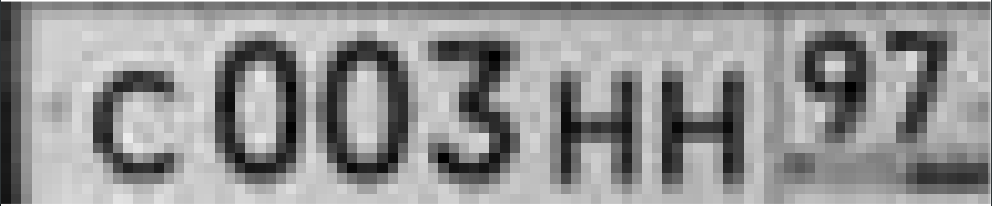
\includegraphics[width=10cm]{content/sr2_two_1.png}};
%     \node (img1) {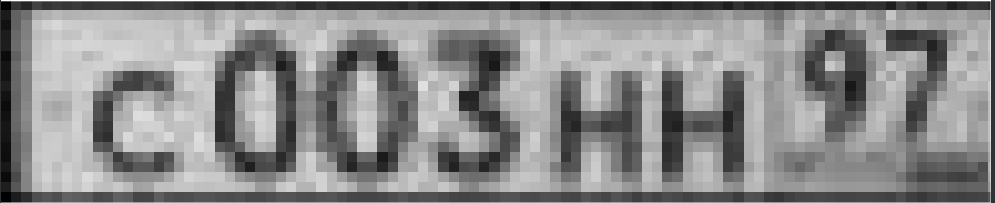
\includegraphics[width=10cm]{content/sr2_two_2.png}};
%   \end{tikzpicture}
  \begin{figure}
    \caption{The results of algorithm FastSR}
    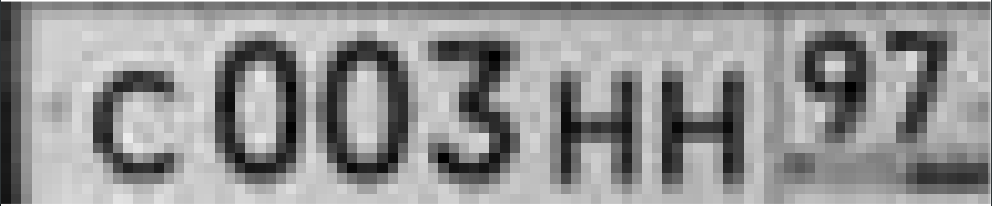
\includegraphics[width=\columnwidth]{content/sr2_two_1.png}\\
  \end{figure}
  \begin{figure}
    \caption{Initial estimation}
    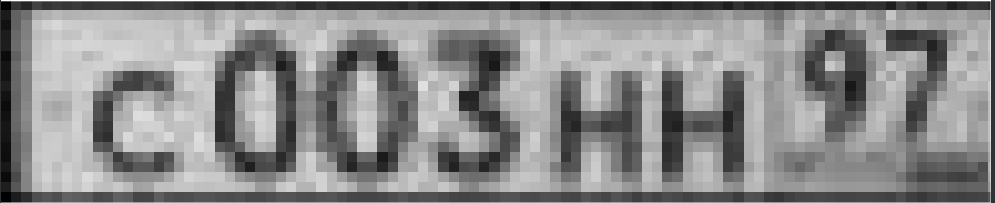
\includegraphics[width=\columnwidth]{content/sr2_two_2.png}
  \end{figure}
 %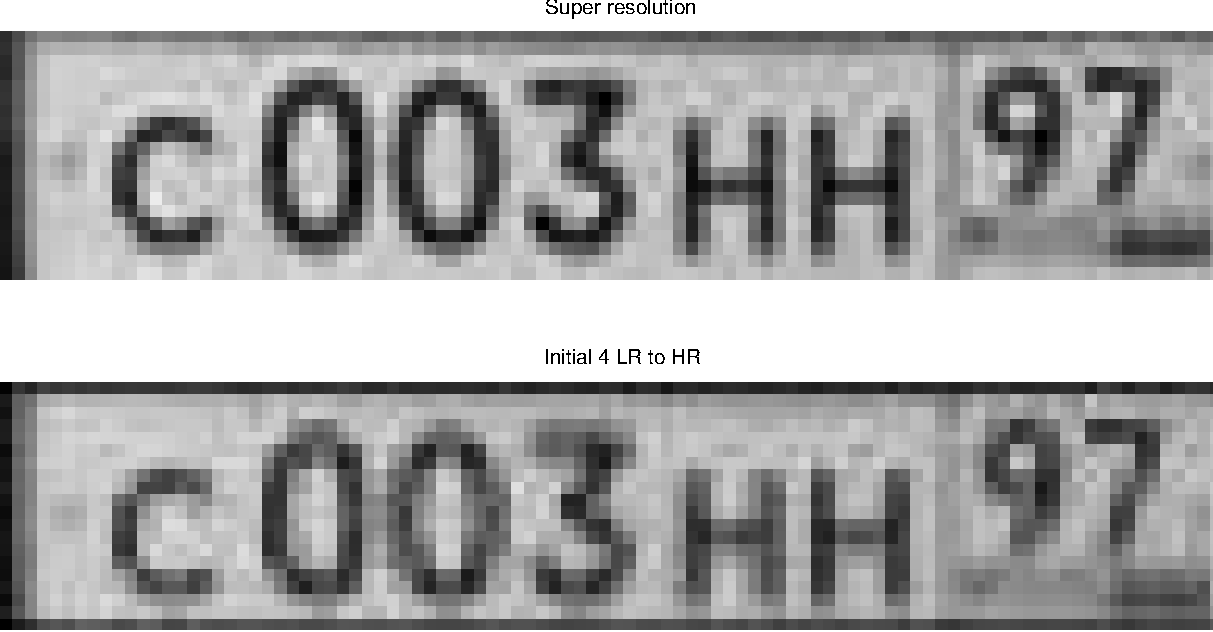
\includegraphics[width=\columnwidth]{content/sr2_two_images.pdf}
\end{frame}

\section{Results}
\begin{frame}{Motion estimation}
  In tests we use true information about shift LR images.

  We research FastSR algorythm result with additive Gaussian noise in warps.
\end{frame}
\bigimg{../text/img/warps_noise.png}{Warp noise test}
\bigimg{../text/img/blur_lambda.png}{Blur test}
\begin{frame}{Conslusion}
 As a result of experiments, it was found that despite the fact that in most cases the first algorithm improves
PSNR, the results of his work is much worse than the second.

  The second algorithm is resistant to noise at the following initial data:
\begin{itemize}
\item robustness shift (up to 0.2 pixel error does not change the result, an error of up to 2 pixels leads to an increase
  in PSNR in comparison with the initial approximation)
\item robustness to noise on the original image (the normal noise with variance $ \sigma = 25 $ for luminance values from 0 to 255)
\item robustness to blur on the original image($\sigma = 1$)
\end{itemize}

\end{frame}


\end{document}
